\documentclass[10pt]{article}
\usepackage[a4paper, margin=1in]{geometry}
\usepackage{kotex} % 한글 사용
\usepackage{enumitem}
\usepackage{amsmath, amssymb, amsfonts}
\usepackage{graphicx}
\usepackage{cprotect} % verbatim을 섹션 등에서 사용하기 위함
\usepackage{hhline} % 표 내의 이중 가로선

% --- 들여쓰기 간격 설정 ---
% \usepackage{indentfirst} % 첫 문단 들여쓰기 활성화
\setlength{\parindent}{0pt} % 들여쓰기 간격 조절
\setlength{\parskip}{1mm} % 문단 간 간격 조절

% --- 제목 정보 설정 ---
\title{\bfseries Final Project - Text Generation}
\author{M1522.006700 확장형 고성능 컴퓨팅 (001)}
\date{2021-15531 컴퓨터공학부 김인호\\ \today}

\linespread{1.2}

% 문서 시작
\begin{document}

% 설정된 정보로 제목 생성
\maketitle

\section{적용한 최적화 기법}

본 과제에서는 LFM2-8B-A1B 모델의 텍스트 생성 성능을 향상시키기 위해 다중 노드와 다중 GPU를 활용한 최적화 기법들을 구현하였다. 주요 접근 방식으로는 노드 간 Data Parallelism(DP)과 GPU 간 Pipeline Parallelism(PP)을 조합하여 사용하였다.

\begin{itemize}
\item \textbf{노드 간 Data Parallelism (DP)}\\
MPI를 활용하여 4개의 계산 노드에 입력 배치를 분할 배치하는 데이터 병렬화 방식을 적용하였다. 각 노드는 전체 모델의 복사본을 가지고 있으며, 서로 다른 배치 샘플에 대해 독립적으로 forward pass를 수행한다. 이를 통해 전체 처리량을 노드 수에 비례하여 향상시킬 수 있었다.

\item \textbf{GPU 간 Pipeline Parallelism (PP)}\\
단일 노드 내에서는 24개의 디코더 레이어를 4개의 GPU에 균등하게 분배(6개씩)하는 Pipeline Parallelism을 적용하였다. 각 GPU는 자신이 담당하는 레이어만 처리하고, 결과를 다음 GPU로 전달하는 파이프라인 방식으로 동작한다. 초기에는 Expert Parallelism(EP)을 시도하였으나, PP가 레이어 간 병렬 처리와 마이크로 배치 파이프라이닝을 통해 더 높은 GPU 활용률을 달성할 수 있어 PP로 전환하였다.

\item \textbf{CUDA 스트림 활용}\\
각 GPU에서 메모리 복사와 커널 실행을 비동기적으로 처리하기 위해 CUDA 스트림을 활용하였다. 이를 통해 GPU 간 통신과 연산이 겹쳐 실행되도록 하여 전체적인 처리 시간을 단축시켰다.

\item \textbf{메모리 최적화}
\begin{itemize}[noitemsep]
    \item \textbf{효율적인 스테이지 간 데이터 전송}: Pipeline Parallelism에서 스테이지 간 hidden state 전달 시 P2P(Peer-to-Peer) DtoD(Device to Device) 복사를 활용하여 메모리 병목을 해소하였다.
    \item \textbf{메모리 재사용}: 중간 텐서들의 메모리 할당과 해제를 최소화하여 메모리 단편화를 줄이고 처리 속도를 향상시켰다.
\end{itemize}

\item \textbf{행렬곱 커널 최적화}: Attention과 Conv 등에서 쓰는 행렬곱 연산에서는 다음과 같은 최적화 기법들을 적용하였다.
\begin{itemize}[noitemsep]
    \item \textbf{Shared Memory Tiling}: 블록 단위로 공유 메모리를 활용한 타일링을 적용하였다.
    \item \textbf{Register Tiling}: 스레드당 연산량을 늘려 레지스터 재사용을 극대화하였다.
    \item \textbf{Double Buffering}: Shared memory에서 계산과 메모리 로드를 겹쳐 수행하였다.
    \item \textbf{Vectorized Memory Access}: float4를 활용한 벡터화된 메모리 접근으로 메모리 대역폭을 향상시켰다.
\end{itemize}

\item \textbf{Buffer Pool을 활용한 메모리 관리}\\
중간 연산 결과를 저장하는 임시 텐서들의 메모리 할당/해제 오버헤드를 줄이기 위해 Buffer Pool을 구현하였다. 각 레이어에서 필요한 중간 텐서들을 미리 할당해 두고 재사용함으로써 메모리 단편화를 방지하고 전체적인 성능을 향상시켰다.

\item \textbf{MoE 최적화}: MoE 블록의 라우팅 과정을 최적화하고, Expert 실행 시 여러 개의 스트림을 활용하여 병렬적으로 MLP를 실행할 수 있도록 하였다.
\begin{itemize}[noitemsep]
    \item \textbf{Warp-level 병렬화}: 32개 Expert에 대한 sigmoid 계산을 warp 내에서 병렬로 처리하였다.
    \item \textbf{Shared memory 기반 Top-K 선택}: 공유 메모리를 활용한 효율적인 Top-K 선택 로직을 구현하였다.
    \item \textbf{Expert 멀티스트림 실행}: 4개의 CUDA 스트림을 활용하여 여러 Expert의 MLP 연산을 병렬로 실행하고, 슬롯 기반 동기화로 오버랩을 극대화하였다.
\end{itemize}

\item \textbf{커널 융합}\\
여러 개의 작은 연산들을 하나의 커널로 융합하여 메모리 접근과 커널 런치 오버헤드를 줄였다.
\begin{itemize}[noitemsep]
    \item \textbf{ShortConv 융합}: transpose → split → convolution → multiply → transpose 연산을 하나의 융합 커널로 구현하였다.
    \item \textbf{Activation 융합}: SiLU 등의 활성화 함수를 행렬곱과 융합하여 처리하였다.
\end{itemize}
\end{itemize}

\section{성능 측정 결과}

최종 구현에서 달성한 성능은 \textbf{424.844621 samples/sec}이다.

\begin{center}
\raisebox{-\height}{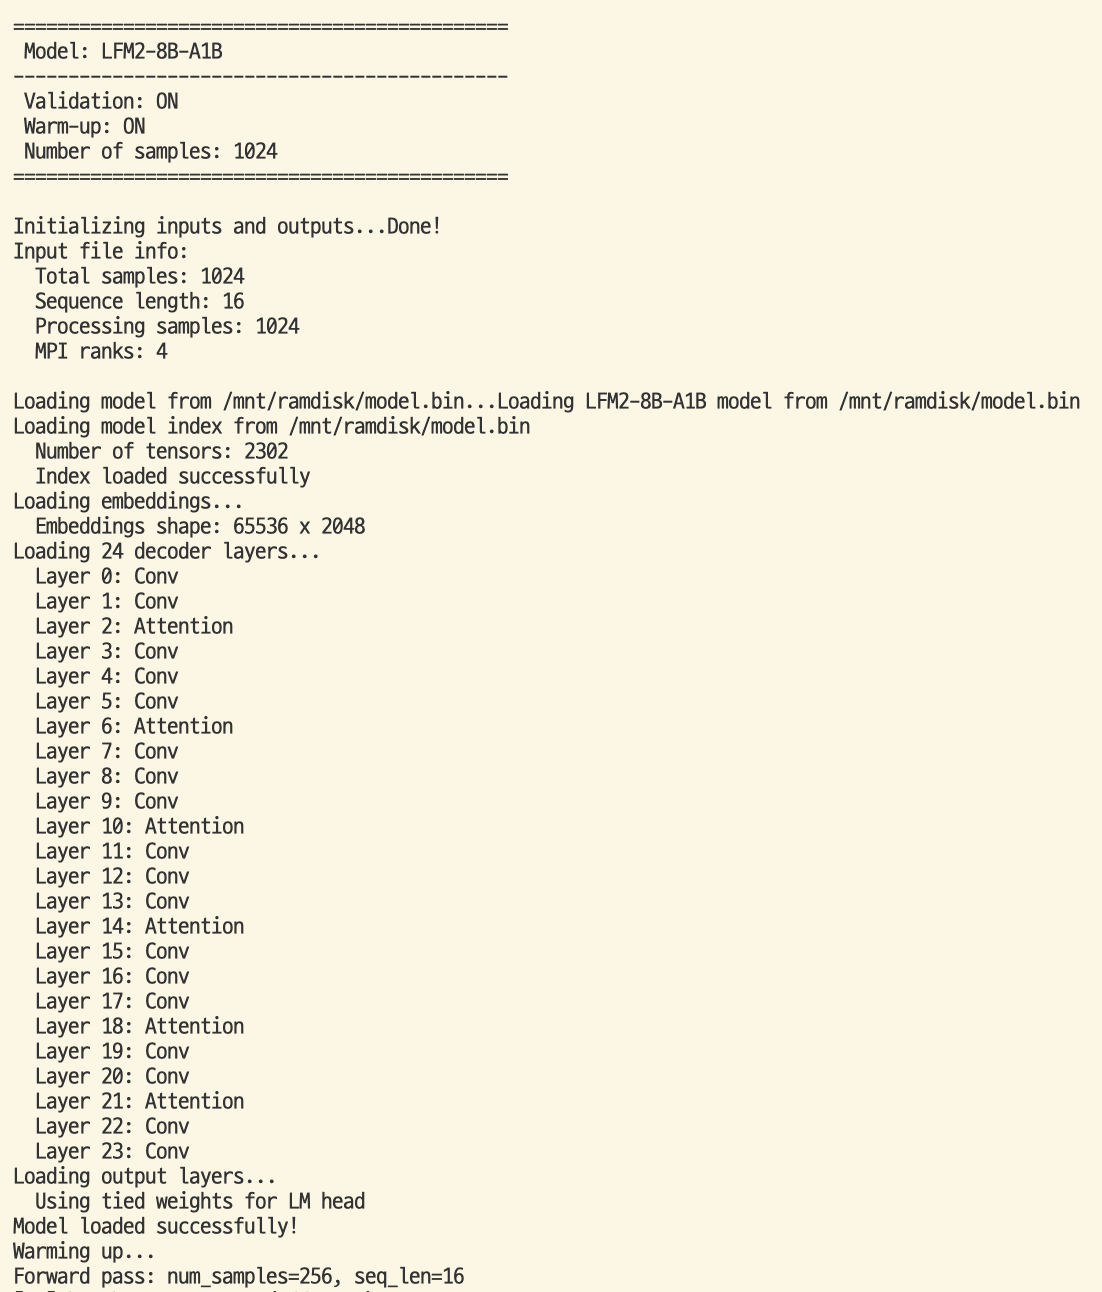
\includegraphics[width=0.45\textwidth]{pp-1.png}}
\raisebox{-\height}{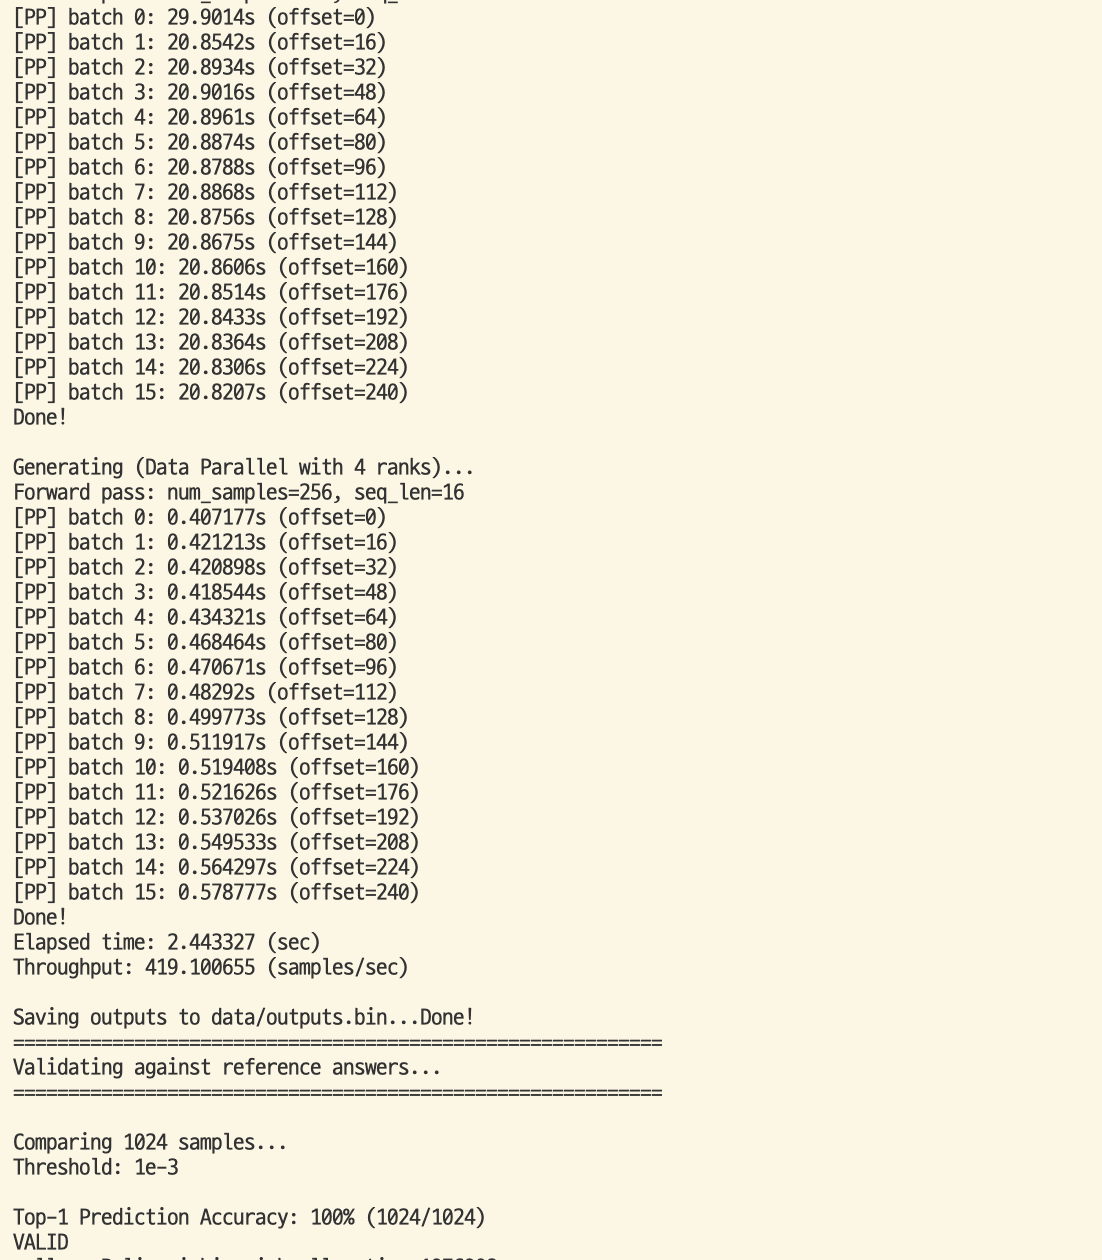
\includegraphics[width=0.45\textwidth]{pp-2.png}}
\end{center}

\textbf{성능 개선 과정}
\begin{itemize}[noitemsep]
\item \textbf{Baseline}: 0.12 samples/sec
\item \textbf{Expert Parallelism 적용}: 0.11 samples/sec (초기 구현에서 오히려 성능 저하)
\item \textbf{MPI Data Parallelism 추가}: 63.9 samples/sec (약 570배 향상)
\item \textbf{커널 최적화}: 81.3 samples/sec (행렬곱, MoE 라우팅, 커널 융합)
\item \textbf{Buffer Pool \& 메모리 최적화}: 128.9 samples/sec (약 58\% 향상)
\item \textbf{메모리 병목 지점 파악 및 수정}: 223.53 samples/sec (약 71\% 향상)
\item \textbf{Pipeline Parallelism으로 전환}: 240.35 samples/sec (약 7.5\% 향상)
\item \textbf{MoE Expert 멀티스트림 활용}: 424.84 samples/sec (약 77\% 향상)
\end{itemize}

검증 정확도는 모든 단계에서 100\%를 유지하여 최적화 과정에서 정확성이 손상되지 않았음을 확인하였다.

\end{document}